\documentclass[tikz,border=3pt]{standalone}
\usepackage[utf8]{inputenc}
\usepackage[T1]{fontenc}
\usepackage{lmodern}
\renewcommand{\familydefault}{\sfdefault}
\usepackage{sansmath}\sansmath
\usepackage{chemfig}
\usepackage{pgfplots}\pgfplotsset{compat=1.18,/pgf/number format/use comma,/pgf/number format/1000 sep={.}}
\usetikzlibrary{arrows.meta,calc,positioning,decorations.pathmorphing,patterns}
% paleta del sitio
\definecolor{nar}{HTML}{E8680C}\definecolor{narc}{HTML}{FFB35C}\definecolor{hielo}{HTML}{FFF3E8}
\definecolor{tinta}{HTML}{1D1D1F}\definecolor{gris}{HTML}{6E6E73}\definecolor{lila}{HTML}{7C5CF0}
\definecolor{azul}{HTML}{2F6FD6}\definecolor{menta}{HTML}{17A673}\definecolor{coral}{HTML}{E8342A}
\begin{document}
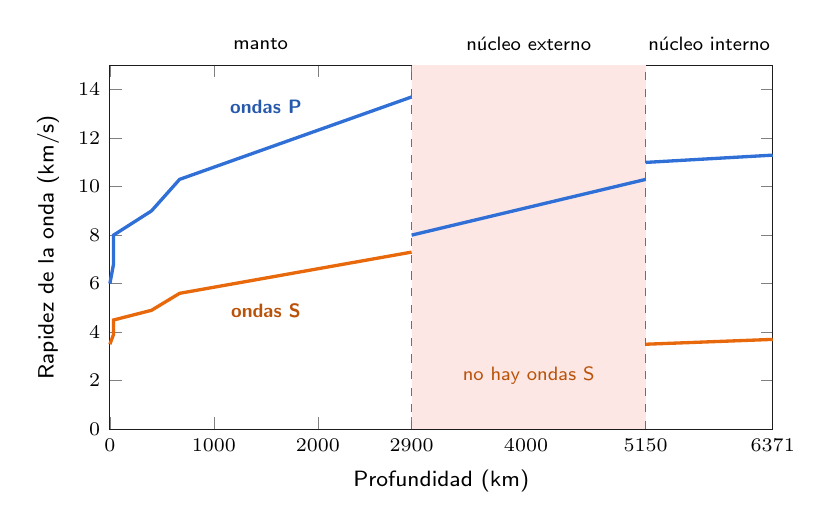
\begin{tikzpicture}[font=\footnotesize]
\begin{axis}[width=10cm,height=6.2cm,xmin=0,xmax=6371,ymin=0,ymax=15,
  xlabel={Profundidad (km)},ylabel={Rapidez de la onda (km/s)},
  xtick={0,1000,2000,2900,4000,5150,6371},
  xticklabel style={/pgf/number format/1000 sep={},font=\scriptsize,rotate=0},
  ytick={0,2,4,6,8,10,12,14},
  axis line style={tinta},tick label style={font=\scriptsize},label style={font=\footnotesize},clip=false]
\fill[coral!12] (axis cs:2900,0) rectangle (axis cs:5150,15);
\draw[gris,dashed] (axis cs:2900,0) -- (axis cs:2900,15);
\draw[gris,dashed] (axis cs:5150,0) -- (axis cs:5150,15);
\addplot[azul,very thick] coordinates {(0,6)(35,6.8)(35,8.0)(400,9.0)(670,10.3)(2900,13.7)};
\addplot[azul,very thick] coordinates {(2900,8.0)(5150,10.3)};
\addplot[azul,very thick] coordinates {(5150,11.0)(6371,11.3)};
\addplot[nar,very thick] coordinates {(0,3.5)(35,3.9)(35,4.5)(400,4.9)(670,5.6)(2900,7.3)};
\addplot[nar,very thick] coordinates {(5150,3.5)(6371,3.7)};
\node[font=\scriptsize\bfseries,text=azul!80!black] at (axis cs:1500,13.3) {ondas P};
\node[font=\scriptsize\bfseries,text=nar!80!black] at (axis cs:1500,4.9) {ondas S};
\node[font=\scriptsize,align=center] at (axis cs:1450,15.9) {manto};
\node[font=\scriptsize,align=center] at (axis cs:4025,15.9) {núcleo externo};
\node[font=\scriptsize,align=center] at (axis cs:5760,15.9) {núcleo interno};
\node[font=\scriptsize,align=center,text=nar!80!black] at (axis cs:4025,2.2) {no hay ondas S};
\end{axis}
\end{tikzpicture}
\end{document}
